 \section{Methodology}
 
% A short summary of how you have represented your system of interest using an ABM and how your model works. You can also use simple flow or state transition diagrams to support your description. You can also refer to relevant code snippets or pseudocode included in an appendix. State, and where possible, justify any assumptions you have made. You should explain in English (as opposed to simply using code), how you have extended the model you have been given in order to investigate the features mentioned. Please refer to assignment description for further guidelines.
 
% Briefly but clearly describe the pertinent components and behavior of the natural system
% Justification of model design appropriate for relevant natural system
% Use of a sensibly structured model description (e.g. the ODD protocol mentioned in the project description).
% Clear statement of any assumptions you have made in developing your model.
 
 \subsection{System Description}
 
At the highest level our ABM consists of one agent, Ants, and an environment that contains their colony, food and then the pheromones that the ants leave behind. We have modelled two types of ants, major workers and minor workers. These are called workers, for major workers, and scouts, minor workers, in this project's code and some of the diagrams.\par
The modelling of our agent 
 
 \begin{figure}[htb]
  \label{fig:ant-highlvl}
  \centering
  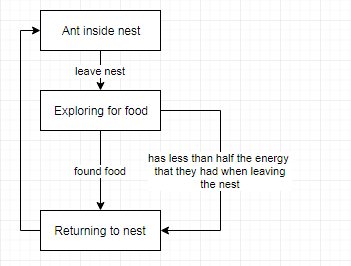
\includegraphics[width=0.5\textwidth]{images/top-level.png}
  \caption{High Level State Diagram for the Ant}
\end{figure}

\begin{figure}[htb]
  \label{fig:ant-highlvl}
  \centering
  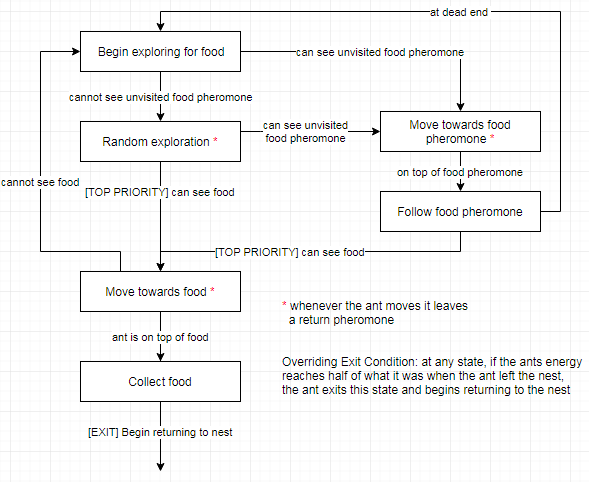
\includegraphics[width=1\textwidth]{images/exploring.png}
  \caption{High Level State Diagram for the Ant}
\end{figure}

\begin{figure}[htb]
  \label{fig:ant-highlvl}
  \centering
  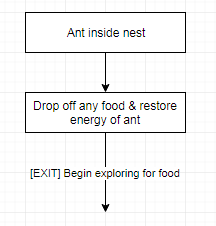
\includegraphics[width=0.4\textwidth]{images/inside-nest.png}
  \caption{High Level State Diagram for the Ant}
\end{figure}

\begin{figure}[htb]
  \label{fig:ant-highlvl}
  \centering
  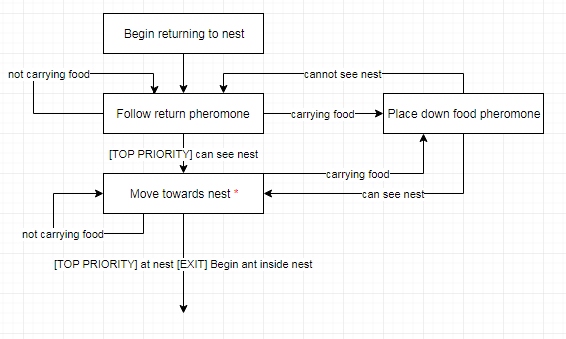
\includegraphics[width=0.5\textwidth]{images/nest-return.png}
  \caption{High Level State Diagram for the Ant}
\end{figure}

The system aims to simulate colonies of ants as they forage for food in a 2d environment. Each colony of ants exists as a single spawn point out of which ants leave to look for food. Each tile contains a value for the strength of food pheromone for each colony. Ants can move from tile to tile to follow pheromone trails towards food. If an ant cannot see a food pheromone trail then they will explore away from the nest for new food sources or food pheromone trails to follow. Ants will reinforce a pheromone trial when they return to the nest with food. To prevent ants being led to depleted food sources, over time these pheromone trails will decay as ants will only reinforce those food pheromone trails that they find food at the end of. 

There exists in this simulation two types of ants, the worker and the scout. The worker ant is capable of carrying more food when it forages and the scout ant cannot carry as much but can move at a slightly faster speed. The simulation can then be configured for each colony to have different proportions of worker and scout ants. 

Timesteps - every 1 minute
Tile Size - 1m x 1m 
Scout Ant Speed - 0.5 meters per minute (8.3 mms-1)
Worker Ant Speed - 0.36 meters per minute (6 mms-1 [source 1]) 

Assumptions made throughout this model include the assumption that a scout ant moves at a speed which is scaled on the speed we found documented of the worker ant (6 mms-1) [source 1]. Due to the diversity of ant movement speeds, the speed of a scout from one species of ant cannot be compared to the speed of a worker from another. By knowing that scout ants move faster however, scaling the worker ant speed gives an approximation of the speed a scout ant of that species would have. Additionally, although ants were modelled to have continuous locations, the environment is grid based and so pheromone trails were located by their tile position. The purpose of this model is that it finds statistical patterns based on the proportion of scout/worker ant populations in each colony, therefore, it is not important that the entire system is modelled in a way that is physically accurate on a ground level, rather that the simulation provides results which are statistically representative of ant colony behaviour. 

Another assumption made was to not model ant encounters, this being where two ants move over each other and cause a slowdown. The reasoning for this was that as according to one study ?direct or interaction effects, has a much smaller effect on walking velocity than does body size? [source 2], therefore the speed of an ant is determined entirely by their body size, which is given as the most important factor. The speed of each ant is determined by them being either the larger and slower worker ant, or the faster but smaller scout ant.

 
 \subsection{Experimental Setup \& Assumptions}



% Things to remember:
% - We have to explain how we've decided on major ants being able to carry additional food based on the fire ants paper by Tschinkel, and why we've chosen that difference
%   - This will probably be along hte lines of 'The paper shows that the body size is 4 times as much as the size of the minor. Because of this, we're *assumimg* that the major can carry ~4 times more"
